% Background: message passing. The generic (phi, bigoplus, psi) form is not Gilmer et al.'s
% notation (they use a sum, M_t and U_t), so it is attributed to Bronstein et al. as well.
% Figure: % Figure: one message-passing update (Eq. eq:mp) and the L-hop receptive field.
% Usage in the thesis: % Figure: one message-passing update (Eq. eq:mp) and the L-hop receptive field.
% Usage in the thesis: % Figure: one message-passing update (Eq. eq:mp) and the L-hop receptive field.
% Usage in the thesis: \input{figures/message_passing}
% Requires in the preamble: \usepackage{tikz}, \usepackage{amsmath}
\begin{figure}[t]
  \centering
  \resizebox{\textwidth}{!}{%
  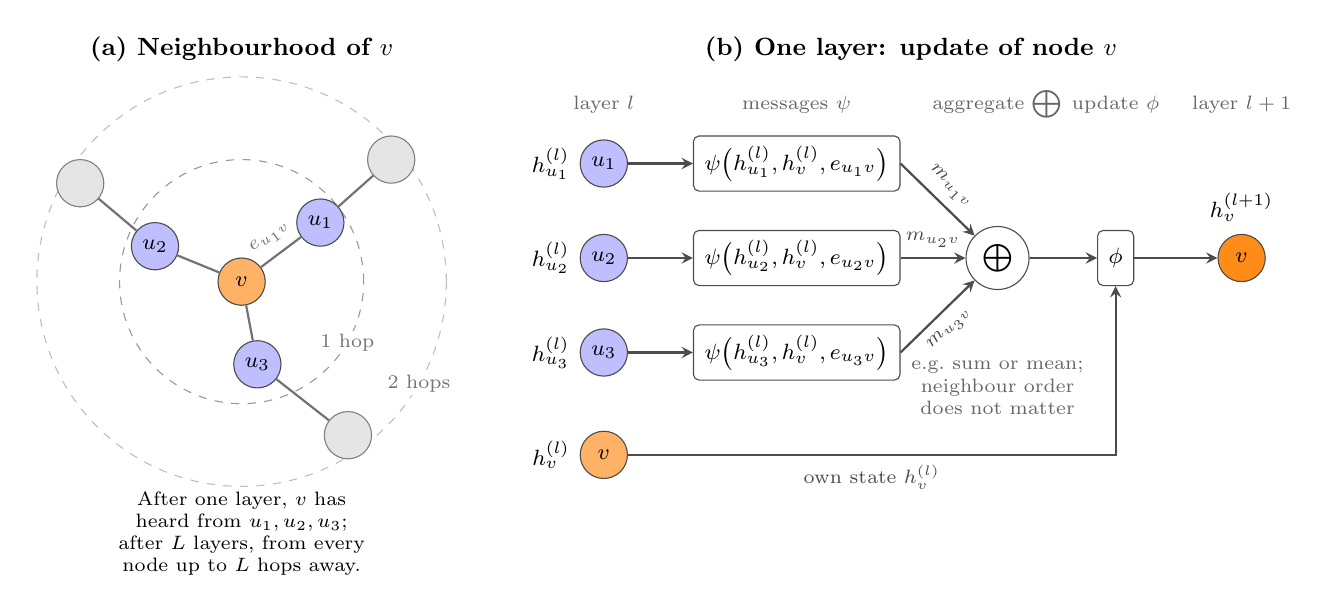
\begin{tikzpicture}[>=stealth,
      every node/.append style={font=\footnotesize},
      vnode/.style={circle, draw=black!70, fill=orange!60, minimum size=6mm, inner sep=0pt},
      unode/.style={circle, draw=black!70, fill=blue!25, minimum size=6mm, inner sep=0pt},
      wnode/.style={circle, draw=black!50, fill=black!10, minimum size=6mm, inner sep=0pt},
      op/.style={draw=black!70, rounded corners=2pt, fill=white, minimum height=7mm, inner xsep=4pt},
      flow/.style={->, black!70, thick}]

    % ---------------- (a) neighbourhood and receptive field ----------------
    \node[font=\small\bfseries] at (0,2.95) {(a) Neighbourhood of $v$};
    \draw[dashed, black!40] (0,0) circle (1.55);
    \draw[dashed, black!25] (0,0) circle (2.6);
    \node[font=\scriptsize, black!55, fill=white, inner sep=1pt] at (-30:1.55) {1 hop};
    \node[font=\scriptsize, black!55, fill=white, inner sep=1pt] at (-30:2.6) {2 hops};

    \node[vnode] (a-v)  at (0,0)        {$v$};
    \node[unode] (a-u1) at (1.0,0.75)   {$u_1$};
    \node[unode] (a-u2) at (-1.1,0.45)  {$u_2$};
    \node[unode] (a-u3) at (0.2,-1.05)  {$u_3$};
    \node[wnode] (a-w1) at (1.9,1.55)   {};
    \node[wnode] (a-w2) at (-2.05,1.25) {};
    \node[wnode] (a-w3) at (1.35,-1.95) {};

    \draw[black!55, thick] (a-v) -- node[midway, above, sloped, font=\scriptsize] {$e_{u_1v}$} (a-u1);
    \foreach \a/\b in {a-v/a-u2, a-v/a-u3, a-u1/a-w1, a-u2/a-w2, a-u3/a-w3}
      \draw[black!55, thick] (\a) -- (\b);

    \node[align=center, text width=5.2cm, font=\scriptsize] at (0,-3.2)
      {After one layer, $v$ has heard from $u_1, u_2, u_3$;\\ after $L$ layers, from every node up to $L$ hops away.};

    % ---------------- (b) one layer's update of node v ----------------
    \begin{scope}[xshift=4.6cm]
      \node[font=\small\bfseries] at (3.9,2.95) {(b) One layer: update of node $v$};
      \foreach \x/\t in {0/layer $l$, 2.45/messages $\psi$, 5.0/aggregate $\bigoplus$, 6.5/update $\phi$, 8.1/layer $l+1$}
        \node[font=\scriptsize, black!60] at (\x,2.25) {\t};

      % neighbour states and v's own state at layer l
      \node[unode] (u1) at (0,1.5)  {$u_1$};
      \node[unode] (u2) at (0,0.3)  {$u_2$};
      \node[unode] (u3) at (0,-0.9) {$u_3$};
      \node[vnode] (v)  at (0,-2.2) {$v$};
      \node[anchor=east] at (u1.west) {$h_{u_1}^{(l)}$};
      \node[anchor=east] at (u2.west) {$h_{u_2}^{(l)}$};
      \node[anchor=east] at (u3.west) {$h_{u_3}^{(l)}$};
      \node[anchor=east] at (v.west)  {$h_{v}^{(l)}$};

      % one message per neighbour
      \node[op] (p1) at (2.45,1.5)  {$\psi\big(h_{u_1}^{(l)}, h_v^{(l)}, e_{u_1v}\big)$};
      \node[op] (p2) at (2.45,0.3)  {$\psi\big(h_{u_2}^{(l)}, h_v^{(l)}, e_{u_2v}\big)$};
      \node[op] (p3) at (2.45,-0.9) {$\psi\big(h_{u_3}^{(l)}, h_v^{(l)}, e_{u_3v}\big)$};
      \draw[flow] (u1) -- (p1);
      \draw[flow] (u2) -- (p2);
      \draw[flow] (u3) -- (p3);

      % permutation-invariant aggregation
      \node[circle, draw=black!70, fill=white, minimum size=8mm, inner sep=0pt] (agg) at (5.0,0.3) {$\bigoplus$};
      \draw[flow] (p1.east) -- node[above, sloped, font=\scriptsize] {$m_{u_1v}$} (agg);
      \draw[flow] (p2.east) -- node[above, font=\scriptsize] {$m_{u_2v}$} (agg);
      \draw[flow] (p3.east) -- node[below, sloped, font=\scriptsize] {$m_{u_3v}$} (agg);
      \node[font=\scriptsize, black!60, align=center] at (5.0,-1.35) {e.g.\ sum or mean;\\ neighbour order\\ does not matter};

      % update: aggregated messages + v's own state
      \node[op] (upd) at (6.5,0.3) {$\phi$};
      \draw[flow] (agg) -- (upd);
      \draw[flow] (v.east) -- node[below, font=\scriptsize] {own state $h_v^{(l)}$} (6.5,-2.2) -- (upd.south);

      % new state
      \node[vnode, fill=orange!90] (out) at (8.1,0.3) {$v$};
      \node[above=1pt] at (out.north) {$h_v^{(l+1)}$};
      \draw[flow] (upd) -- (out);
    \end{scope}
  \end{tikzpicture}}
  \caption{Message passing (Eq.~\eqref{eq:mp}). (a)~Node $v$ (orange), its neighbours (blue) and
    nodes two hops away (grey); stacking layers widens the neighbourhood $v$ receives information
    from. (b)~One layer: each neighbour $u$ sends a message $\psi\big(h_u^{(l)}, h_v^{(l)}, e_{uv}\big)$,
    the messages are combined by a permutation-invariant aggregation $\bigoplus$, and the update
    $\phi$ combines the result with $v$'s own state to give $h_v^{(l+1)}$. All nodes are updated
    this way in parallel, with the same $\psi$ and $\phi$.}
  \label{fig:mp}
\end{figure}

% Requires in the preamble: \usepackage{tikz}, \usepackage{amsmath}
\begin{figure}[t]
  \centering
  \resizebox{\textwidth}{!}{%
  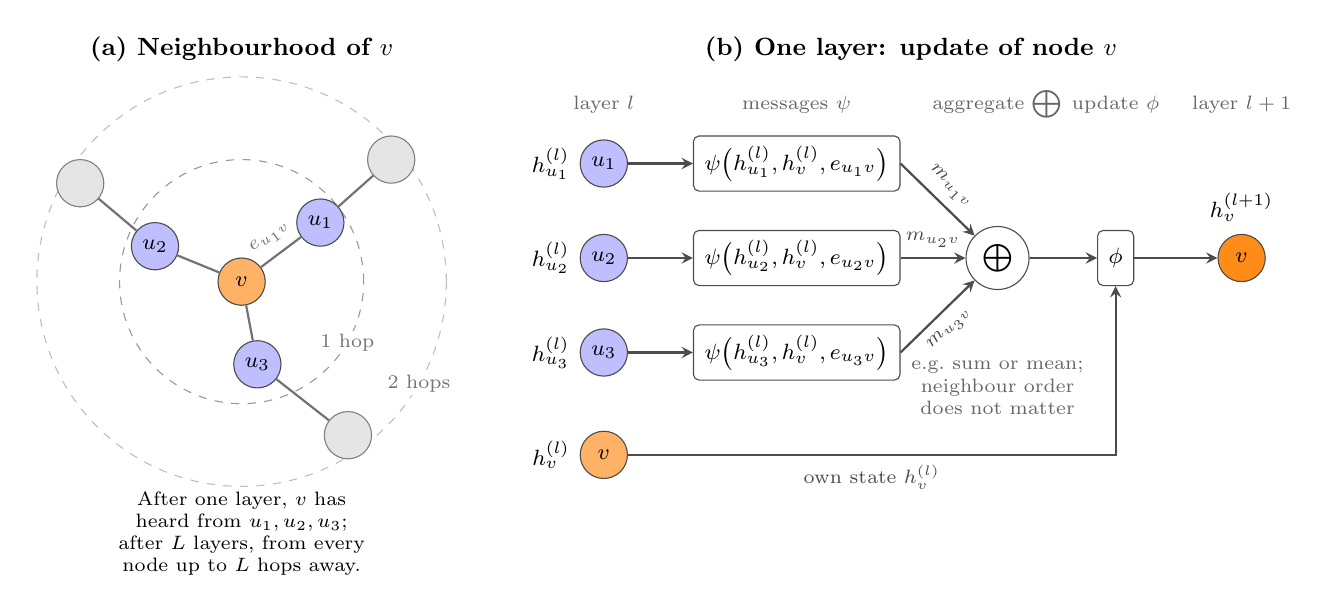
\begin{tikzpicture}[>=stealth,
      every node/.append style={font=\footnotesize},
      vnode/.style={circle, draw=black!70, fill=orange!60, minimum size=6mm, inner sep=0pt},
      unode/.style={circle, draw=black!70, fill=blue!25, minimum size=6mm, inner sep=0pt},
      wnode/.style={circle, draw=black!50, fill=black!10, minimum size=6mm, inner sep=0pt},
      op/.style={draw=black!70, rounded corners=2pt, fill=white, minimum height=7mm, inner xsep=4pt},
      flow/.style={->, black!70, thick}]

    % ---------------- (a) neighbourhood and receptive field ----------------
    \node[font=\small\bfseries] at (0,2.95) {(a) Neighbourhood of $v$};
    \draw[dashed, black!40] (0,0) circle (1.55);
    \draw[dashed, black!25] (0,0) circle (2.6);
    \node[font=\scriptsize, black!55, fill=white, inner sep=1pt] at (-30:1.55) {1 hop};
    \node[font=\scriptsize, black!55, fill=white, inner sep=1pt] at (-30:2.6) {2 hops};

    \node[vnode] (a-v)  at (0,0)        {$v$};
    \node[unode] (a-u1) at (1.0,0.75)   {$u_1$};
    \node[unode] (a-u2) at (-1.1,0.45)  {$u_2$};
    \node[unode] (a-u3) at (0.2,-1.05)  {$u_3$};
    \node[wnode] (a-w1) at (1.9,1.55)   {};
    \node[wnode] (a-w2) at (-2.05,1.25) {};
    \node[wnode] (a-w3) at (1.35,-1.95) {};

    \draw[black!55, thick] (a-v) -- node[midway, above, sloped, font=\scriptsize] {$e_{u_1v}$} (a-u1);
    \foreach \a/\b in {a-v/a-u2, a-v/a-u3, a-u1/a-w1, a-u2/a-w2, a-u3/a-w3}
      \draw[black!55, thick] (\a) -- (\b);

    \node[align=center, text width=5.2cm, font=\scriptsize] at (0,-3.2)
      {After one layer, $v$ has heard from $u_1, u_2, u_3$;\\ after $L$ layers, from every node up to $L$ hops away.};

    % ---------------- (b) one layer's update of node v ----------------
    \begin{scope}[xshift=4.6cm]
      \node[font=\small\bfseries] at (3.9,2.95) {(b) One layer: update of node $v$};
      \foreach \x/\t in {0/layer $l$, 2.45/messages $\psi$, 5.0/aggregate $\bigoplus$, 6.5/update $\phi$, 8.1/layer $l+1$}
        \node[font=\scriptsize, black!60] at (\x,2.25) {\t};

      % neighbour states and v's own state at layer l
      \node[unode] (u1) at (0,1.5)  {$u_1$};
      \node[unode] (u2) at (0,0.3)  {$u_2$};
      \node[unode] (u3) at (0,-0.9) {$u_3$};
      \node[vnode] (v)  at (0,-2.2) {$v$};
      \node[anchor=east] at (u1.west) {$h_{u_1}^{(l)}$};
      \node[anchor=east] at (u2.west) {$h_{u_2}^{(l)}$};
      \node[anchor=east] at (u3.west) {$h_{u_3}^{(l)}$};
      \node[anchor=east] at (v.west)  {$h_{v}^{(l)}$};

      % one message per neighbour
      \node[op] (p1) at (2.45,1.5)  {$\psi\big(h_{u_1}^{(l)}, h_v^{(l)}, e_{u_1v}\big)$};
      \node[op] (p2) at (2.45,0.3)  {$\psi\big(h_{u_2}^{(l)}, h_v^{(l)}, e_{u_2v}\big)$};
      \node[op] (p3) at (2.45,-0.9) {$\psi\big(h_{u_3}^{(l)}, h_v^{(l)}, e_{u_3v}\big)$};
      \draw[flow] (u1) -- (p1);
      \draw[flow] (u2) -- (p2);
      \draw[flow] (u3) -- (p3);

      % permutation-invariant aggregation
      \node[circle, draw=black!70, fill=white, minimum size=8mm, inner sep=0pt] (agg) at (5.0,0.3) {$\bigoplus$};
      \draw[flow] (p1.east) -- node[above, sloped, font=\scriptsize] {$m_{u_1v}$} (agg);
      \draw[flow] (p2.east) -- node[above, font=\scriptsize] {$m_{u_2v}$} (agg);
      \draw[flow] (p3.east) -- node[below, sloped, font=\scriptsize] {$m_{u_3v}$} (agg);
      \node[font=\scriptsize, black!60, align=center] at (5.0,-1.35) {e.g.\ sum or mean;\\ neighbour order\\ does not matter};

      % update: aggregated messages + v's own state
      \node[op] (upd) at (6.5,0.3) {$\phi$};
      \draw[flow] (agg) -- (upd);
      \draw[flow] (v.east) -- node[below, font=\scriptsize] {own state $h_v^{(l)}$} (6.5,-2.2) -- (upd.south);

      % new state
      \node[vnode, fill=orange!90] (out) at (8.1,0.3) {$v$};
      \node[above=1pt] at (out.north) {$h_v^{(l+1)}$};
      \draw[flow] (upd) -- (out);
    \end{scope}
  \end{tikzpicture}}
  \caption{Message passing (Eq.~\eqref{eq:mp}). (a)~Node $v$ (orange), its neighbours (blue) and
    nodes two hops away (grey); stacking layers widens the neighbourhood $v$ receives information
    from. (b)~One layer: each neighbour $u$ sends a message $\psi\big(h_u^{(l)}, h_v^{(l)}, e_{uv}\big)$,
    the messages are combined by a permutation-invariant aggregation $\bigoplus$, and the update
    $\phi$ combines the result with $v$'s own state to give $h_v^{(l+1)}$. All nodes are updated
    this way in parallel, with the same $\psi$ and $\phi$.}
  \label{fig:mp}
\end{figure}

% Requires in the preamble: \usepackage{tikz}, \usepackage{amsmath}
\begin{figure}[t]
  \centering
  \resizebox{\textwidth}{!}{%
  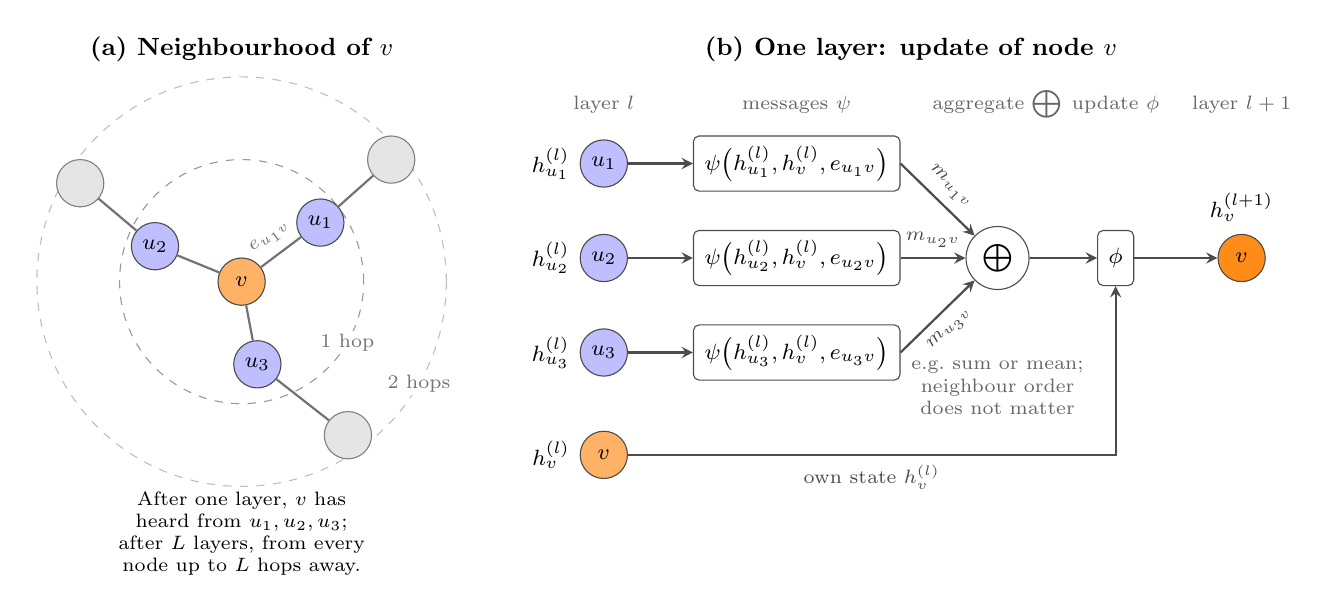
\begin{tikzpicture}[>=stealth,
      every node/.append style={font=\footnotesize},
      vnode/.style={circle, draw=black!70, fill=orange!60, minimum size=6mm, inner sep=0pt},
      unode/.style={circle, draw=black!70, fill=blue!25, minimum size=6mm, inner sep=0pt},
      wnode/.style={circle, draw=black!50, fill=black!10, minimum size=6mm, inner sep=0pt},
      op/.style={draw=black!70, rounded corners=2pt, fill=white, minimum height=7mm, inner xsep=4pt},
      flow/.style={->, black!70, thick}]

    % ---------------- (a) neighbourhood and receptive field ----------------
    \node[font=\small\bfseries] at (0,2.95) {(a) Neighbourhood of $v$};
    \draw[dashed, black!40] (0,0) circle (1.55);
    \draw[dashed, black!25] (0,0) circle (2.6);
    \node[font=\scriptsize, black!55, fill=white, inner sep=1pt] at (-30:1.55) {1 hop};
    \node[font=\scriptsize, black!55, fill=white, inner sep=1pt] at (-30:2.6) {2 hops};

    \node[vnode] (a-v)  at (0,0)        {$v$};
    \node[unode] (a-u1) at (1.0,0.75)   {$u_1$};
    \node[unode] (a-u2) at (-1.1,0.45)  {$u_2$};
    \node[unode] (a-u3) at (0.2,-1.05)  {$u_3$};
    \node[wnode] (a-w1) at (1.9,1.55)   {};
    \node[wnode] (a-w2) at (-2.05,1.25) {};
    \node[wnode] (a-w3) at (1.35,-1.95) {};

    \draw[black!55, thick] (a-v) -- node[midway, above, sloped, font=\scriptsize] {$e_{u_1v}$} (a-u1);
    \foreach \a/\b in {a-v/a-u2, a-v/a-u3, a-u1/a-w1, a-u2/a-w2, a-u3/a-w3}
      \draw[black!55, thick] (\a) -- (\b);

    \node[align=center, text width=5.2cm, font=\scriptsize] at (0,-3.2)
      {After one layer, $v$ has heard from $u_1, u_2, u_3$;\\ after $L$ layers, from every node up to $L$ hops away.};

    % ---------------- (b) one layer's update of node v ----------------
    \begin{scope}[xshift=4.6cm]
      \node[font=\small\bfseries] at (3.9,2.95) {(b) One layer: update of node $v$};
      \foreach \x/\t in {0/layer $l$, 2.45/messages $\psi$, 5.0/aggregate $\bigoplus$, 6.5/update $\phi$, 8.1/layer $l+1$}
        \node[font=\scriptsize, black!60] at (\x,2.25) {\t};

      % neighbour states and v's own state at layer l
      \node[unode] (u1) at (0,1.5)  {$u_1$};
      \node[unode] (u2) at (0,0.3)  {$u_2$};
      \node[unode] (u3) at (0,-0.9) {$u_3$};
      \node[vnode] (v)  at (0,-2.2) {$v$};
      \node[anchor=east] at (u1.west) {$h_{u_1}^{(l)}$};
      \node[anchor=east] at (u2.west) {$h_{u_2}^{(l)}$};
      \node[anchor=east] at (u3.west) {$h_{u_3}^{(l)}$};
      \node[anchor=east] at (v.west)  {$h_{v}^{(l)}$};

      % one message per neighbour
      \node[op] (p1) at (2.45,1.5)  {$\psi\big(h_{u_1}^{(l)}, h_v^{(l)}, e_{u_1v}\big)$};
      \node[op] (p2) at (2.45,0.3)  {$\psi\big(h_{u_2}^{(l)}, h_v^{(l)}, e_{u_2v}\big)$};
      \node[op] (p3) at (2.45,-0.9) {$\psi\big(h_{u_3}^{(l)}, h_v^{(l)}, e_{u_3v}\big)$};
      \draw[flow] (u1) -- (p1);
      \draw[flow] (u2) -- (p2);
      \draw[flow] (u3) -- (p3);

      % permutation-invariant aggregation
      \node[circle, draw=black!70, fill=white, minimum size=8mm, inner sep=0pt] (agg) at (5.0,0.3) {$\bigoplus$};
      \draw[flow] (p1.east) -- node[above, sloped, font=\scriptsize] {$m_{u_1v}$} (agg);
      \draw[flow] (p2.east) -- node[above, font=\scriptsize] {$m_{u_2v}$} (agg);
      \draw[flow] (p3.east) -- node[below, sloped, font=\scriptsize] {$m_{u_3v}$} (agg);
      \node[font=\scriptsize, black!60, align=center] at (5.0,-1.35) {e.g.\ sum or mean;\\ neighbour order\\ does not matter};

      % update: aggregated messages + v's own state
      \node[op] (upd) at (6.5,0.3) {$\phi$};
      \draw[flow] (agg) -- (upd);
      \draw[flow] (v.east) -- node[below, font=\scriptsize] {own state $h_v^{(l)}$} (6.5,-2.2) -- (upd.south);

      % new state
      \node[vnode, fill=orange!90] (out) at (8.1,0.3) {$v$};
      \node[above=1pt] at (out.north) {$h_v^{(l+1)}$};
      \draw[flow] (upd) -- (out);
    \end{scope}
  \end{tikzpicture}}
  \caption{Message passing (Eq.~\eqref{eq:mp}). (a)~Node $v$ (orange), its neighbours (blue) and
    nodes two hops away (grey); stacking layers widens the neighbourhood $v$ receives information
    from. (b)~One layer: each neighbour $u$ sends a message $\psi\big(h_u^{(l)}, h_v^{(l)}, e_{uv}\big)$,
    the messages are combined by a permutation-invariant aggregation $\bigoplus$, and the update
    $\phi$ combines the result with $v$'s own state to give $h_v^{(l+1)}$. All nodes are updated
    this way in parallel, with the same $\psi$ and $\phi$.}
  \label{fig:mp}
\end{figure}
 (labels m_{uv} defined in the last sentence).
A graph neural network learns a representation for each node by repeatedly combining its features
with those of its neighbours. In the message passing framework of \citet{gilmer2017mpnn}, written
here in the more general form of \citet{bronstein2021geometric} with an arbitrary
permutation-invariant aggregation $\bigoplus$, layer $l+1$ computes
\begin{equation}
h_v^{(l+1)} = \phi\!\left( h_v^{(l)},\; \bigoplus_{u \in \mathcal{N}(v)} \psi\!\left( h_u^{(l)}, h_v^{(l)}, e_{uv} \right) \right),
\label{eq:mp}
\end{equation}
where $h_v^{(l)}$ is the state of node $v$ after $l$ layers, $\mathcal{N}(v)$ its neighbours,
$e_{uv}$ an optional edge feature, $\psi$ a message function, $\bigoplus$ a permutation-invariant
aggregation such as a sum or mean, and $\phi$ an update function; we write
$m_{uv} = \psi\big(h_u^{(l)}, h_v^{(l)}, e_{uv}\big)$ for the message from $u$ to $v$
(Figure~\ref{fig:mp}). Stacking $L$ layers lets each node receive information from nodes up to $L$
hops away.
